% DO NOT COMPILE THIS FILE DIRECTLY!
% This is included by the other .tex files.

\begin{frame}
\titlepage
\end{frame}

\begin{frame}
  \frametitle{about CIRCL}
  
\includegraphics[scale=0.4]{circl.png}
  \begin{itemize}
    \item The Computer Incident Response Center Luxembourg (CIRCL) is a government-driven initiative designed to provide a systematic response facility to computer security threats and incidents. CIRCL is the CERT for the private sector, communes and non-governmental entities in Luxembourg and is operated by securitymadein.lu g.i.e.
  \end{itemize}
\end{frame}

\begin{frame}
  \frametitle{MISP and CIRCL}
  \begin{itemize}
    \item CIRCL is mandated by the Ministry of Economy and acting as the Luxembourg National CERT for private sector.
    \item CIRCL leads the development of the Open Source MISP threat intelligence platform which is used by many military or intelligence communities, private companies, financial sector, National CERTs and LEAs globally.
    \item {\bf CIRCL runs multiple large MISP communities performing active daily threat-intelligence sharing}.
  \end{itemize}
\end{frame}

\begin{frame}
  \frametitle{The aim of this presentation}
  \begin{itemize}
     \item To give some insight into what sort of an evolution of our various communities' have gone through as observed over the past ~8 years
     \item Show the importance of strong contextualisation...
     \item ...and how that can be leveraged when trying to make our data actionable
  \end{itemize}
\end{frame}

\begin{frame}
  \frametitle{Development based on practical user feedback}
  \begin{itemize}
    \item There are many different types of users of an information sharing platform like MISP:
    \begin{itemize}
      \item {\bf Malware reversers} willing to share indicators of analysis with respective colleagues.
      \item {\bf Security analysts} searching, validating and using indicators in operational security.
      \item {\bf Intelligence analysts} gathering information about specific adversary groups.
      \item {\bf Law-enforcement} relying on indicators to support or bootstrap their DFIR cases.
      \item {\bf Risk analysis teams} willing to know about the new threats, likelyhood and occurences.
      \item {\bf Fraud analysts} willing to share financial indicators to detect financial frauds.
    \end{itemize}
  \end{itemize}
\end{frame}

\begin{frame}
  \frametitle{The initial scope of MISP}
  \begin{itemize}
    \item {\bf Extract information} during the analysis process
    \item Store and {\bf correlate} these datapoints
    \item {\bf Share} the data with partners
    \item Focus on technical indicators: IP, domain, hostname, hashes, filename, pattern in file/memory/traffic
    \item Generate protective signatures out of the data: snort, suricata, OpenIOC
  \end{itemize}
\end{frame}

\begin{frame}
  \frametitle{Initial workflow}
  \begin{center}
    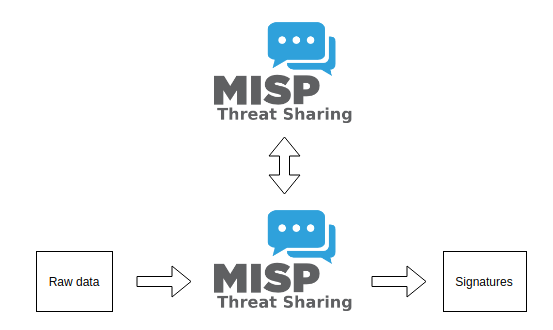
\includegraphics[scale=0.4]{workflow_initial.png}
  \end{center}
\end{frame}

\begin{frame}
  \frametitle{Why was it so simplistic?}
  \begin{itemize}
    \item This was both a reflection of our maturity as a community
    \begin{itemize}
      \item Capabilities for {\bf extracting} information
      \item Capabilities for {\bf utilising} the information
      \item Lack of {\bf willingness} to share context
      \item Lack of {\bf co-operation} between teams doing technical analysis/monitoring and threat-intel
    \end{itemize}
    \item The more growth we saw in maturity, the more we tried to match it with our data-model, often against pushback
  \end{itemize}
\end{frame}

\begin{frame}
\frametitle{The growing need to contextualise data}
\begin{itemize}
       \item There were separate factors that made our data-sets less and less useful for detection/defense in general
        \begin{itemize}
                \item {\bf Growth of our communities} different organisations with different objectives often lead to different quality data or data with a different focus
                \item More advanced protective methods relied on knowing {\bf why certain information is of interest}, rather than just being fed raw data
                \item {\bf False positive management} became more pivotal - and more importantly more diverse based on different use-cases
                \item {\bf TTPs and aggregate information} in general were much more important to threat intel analysts and those dealing with risk assessment than raw data
                \item Due to the increased data volumes, depending on the tools being fed there was a growing need to be able to prioritise
        \end{itemize}
\end{itemize}
\end{frame}

\begin{frame}
\frametitle{Our initial solution}
\begin{itemize}
       \item Allow users to {\bf tag any information} created in MISP
       \item We wanted to be {\bf lax with what we accept} in terms of data, but be {\bf strict on what we fed to our tools}, with strong filter options
       \item We had some ideas on how to potentially move forward...
\end{itemize}
\end{frame}

\begin{frame}
\frametitle{Our initial failures}
\begin{itemize}
       \item Try to capture different aspects of contextualisation into {\bf normalised values} (threat level, source reliability, etc)
        \begin{itemize}
                \item Didn't scale with needs other than our own
                \item Incorporating new types of contextualisation would mean {\bf the modification of the software}
                \item Getting communities with {\bf established naming conventions} to use anything but their go-to vocabularies was a pipe-dream
                \item Heated arguments over numeric conversions
        \end{itemize}
\end{itemize}
\end{frame}

\begin{frame}
  \frametitle{Human creativity}
  \begin{itemize}
    \item We tried an alternate approach instead: Free tagging
    \begin{itemize}
      \item Result was spectacularly painful, at least 7 different ways to spell tlp:amber
      \item No canonisation for common terms lead to tagging ultimately becoming a highly flawed tool for filtering within a sharing community
    \end{itemize}
  \end{itemize}
  \begin{center}
    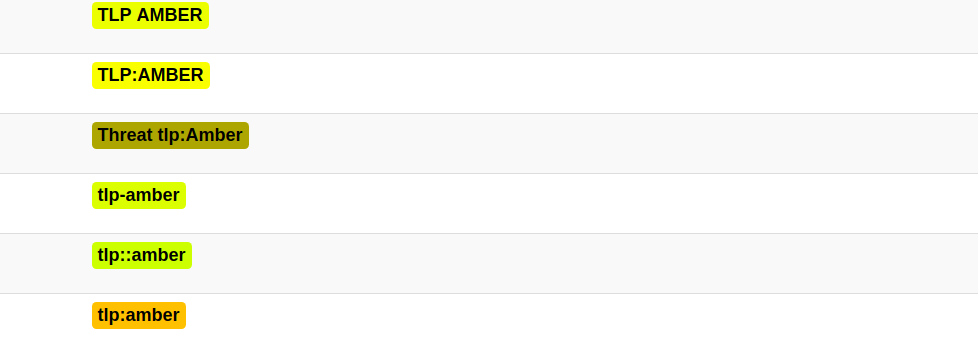
\includegraphics[scale=0.24]{creativity.png}
  \end{center}
\end{frame}

\begin{frame}
\frametitle{How we ended up tackling the issue more successfuly}
\begin{itemize}
       \item We ended up with a mixed approach, currently implemented by the MISP-taxonomy system
        \begin{itemize}
                \item Taxonomies are {\bf vocabularies} of known tags
                \item Tags would be in a {\bf triple tag format} (namespace:predicate=''value'')
                \item Each taxonomy tag could have an optional normalised {\bf numerical value} (0-100)
                \item Create your own taxonomies, recipients should be able to use data you tag with them
                \item Avoid any coding, stick to {\bf JSON}
        \end{itemize}
        \item Massive success, approaching 100 taxonomies
        \item Organisations can solve their own issues without having to rely on us
\end{itemize}
\end{frame}

\begin{frame}
\frametitle{We were still missing something...}
\begin{itemize}
       \item Taxonomy tags were in some cases non self-explanatory
       \item Example: universal understanding of tlp:green vs APT 28
       \item For the latter, a single string was ill-suited
       \item So we needed something new in addition to taxonomies - Galaxies
        \begin{itemize}
                \item Community driven knowledge-base libraries used as tags
                \item Including descriptions, links, synonyms, meta information, etc. 
                \item Goal was to keep it simple and make it reusable
                \item Internally it works the exact same way as taxonomies
        \end{itemize}
\end{itemize}
\end{frame}

\begin{frame}
\frametitle{Broadening the scope of what sort of context we are interested in}
\begin{itemize}
       \item {\bf Who} can receive our data? {\bf What} can they do with it?
       \item {\bf Data accuracy, source reliability}
       \item {\bf Why} is this data relevant to us?
       \item {\bf Who} do we think is behind it, {\bf what tools} were used?
       \item What sort of {\bf motivations} are we dealing with? Who are the {\bf targets}?
       \item How can we {\bf block/detect/remediate} the attack?
       \item What sort of {\bf impact} are we dealing with?
\end{itemize}
\end{frame}

\begin{frame}
\frametitle{Parallel to the contextualisation efforts: False positive handling}
\begin{itemize}
        \item One of the most common criticisms: {\bf low quality / false positive} prone information being shared
        \item Lead to {\bf alert-fatigue}, organisations not using the data in any automated fashion
        \item Could you kick organisation xy out of the community?
        \item False positives are often blatantly obvious - {\bf can't we encode this knowledge}?
        \item {\bf Warninglist system}\footnote{\url{https://github.com/MISP/misp-warninglists}} aims to do that
        \item Predefined lists of well-known indicators which are often false-positives like RFC1918 networks, public DNS resolver are included by default
\end{itemize}
\end{frame}

\begin{frame}
  \frametitle{More complex data-structures for a modern age}
  \begin{itemize}
    \item Atomic attributes were a great starting point, but lacking in many aspects
    \item {\bf MISP objects}\footnote{\url{https://github.com/MISP/misp-objects}} system
    \begin{itemize}
      \item Simple {\bf templating} approach
      \item Use templating to build more complex structures
      \item Decouple it from the core, allow users to {\bf define their own} structures
      \item MISP should understand the data without knowing the templates
      \item Massive caveat: {\bf Building blocks have to be MISP attribute types}
      \item Allow {\bf relationships} to be built between objects
    \end{itemize}
  \end{itemize}
\end{frame}

\begin{frame}
  \frametitle{Supporting specific datamodel}
  \begin{center}
    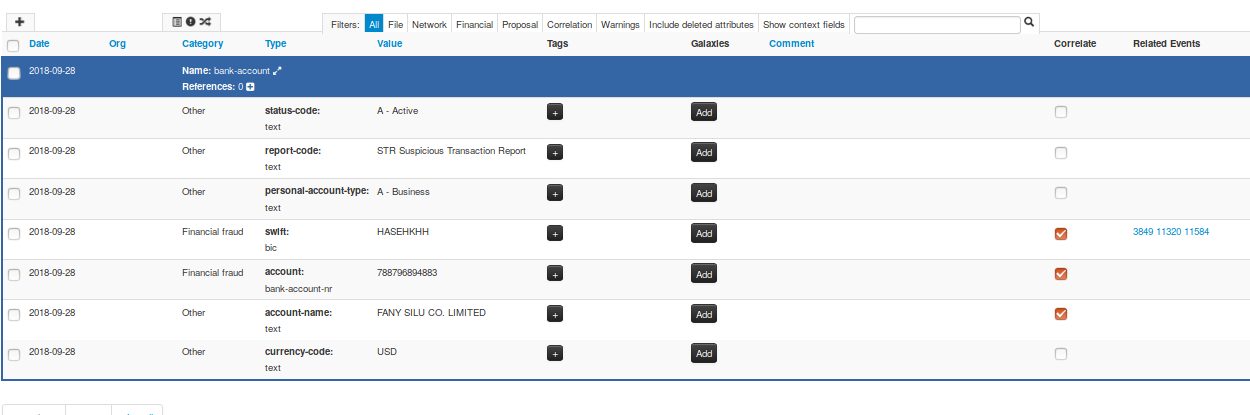
\includegraphics[scale=0.24]{bankaccount.png}
  \end{center}
  \begin{center}
    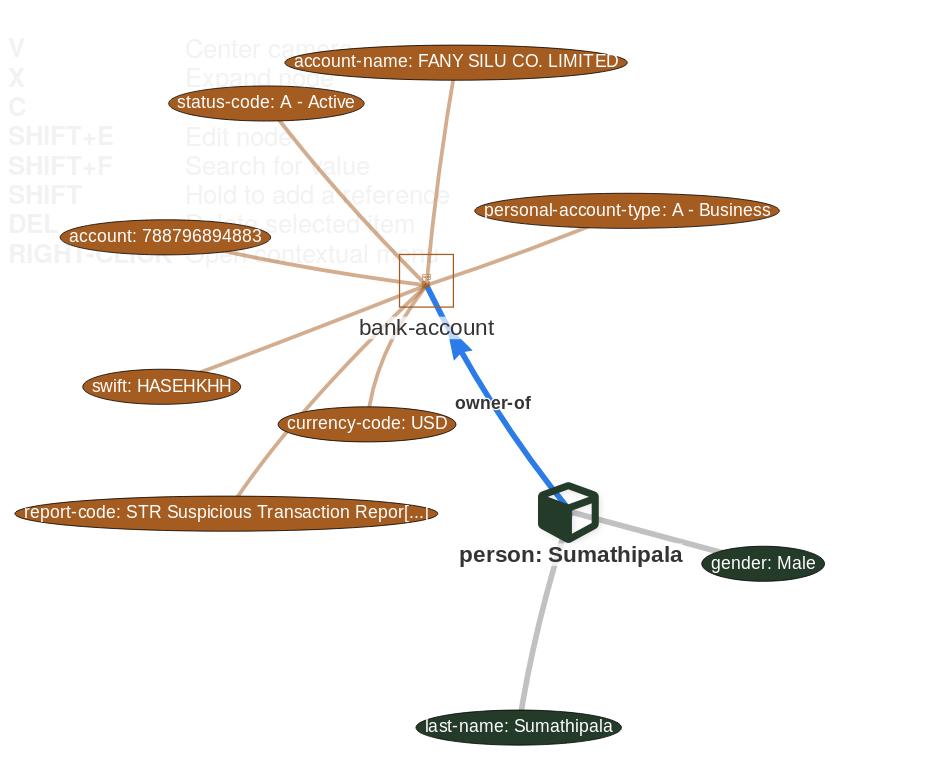
\includegraphics[scale=0.18]{bankview.png}
  \end{center}
\end{frame}

\begin{frame}
  \frametitle{Continuous feedback loop}
  \begin{itemize}
    \item Data ingested by MISP was in a sense frozen in time
    \item We had a creation data, but lacked a way to use the output of our detection
    \item Lead to the introduction of the {\bf Sighting system}
    \item The community could sight indicators and convey the time of sighting
    \item Potentially powerful tool for IoC lifecycle management, clumsy query implementation default
  \end{itemize}
\end{frame}

\begin{frame}
  \frametitle{Supporting specific datamodel}
  \begin{center}
    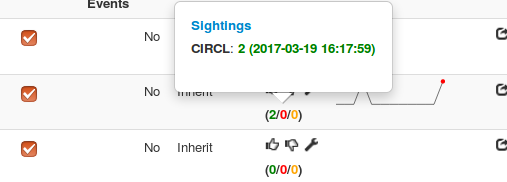
\includegraphics[scale=0.3]{sighting-n.png}
  \end{center}
  \begin{center}
    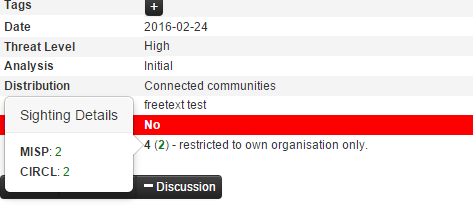
\includegraphics[scale=0.34]{Sightings2.PNG}
  \end{center}  
\end{frame}

\begin{frame}
  \frametitle{Making use of all this context}
  \begin{itemize}
    \item Most obvious goal: Improve the way we query data
    \begin{itemize}
      \item Unified all export APIs
      \item Incorporate all contextualisation options into {\bf API filters}
      \item Allow for an {\bf on-demand} way of {\bf excluding potential false positives}
      \item Allow users to easily {\bf build their own} export modules feed their various tools
    \end{itemize}
  \end{itemize}
\end{frame}

\begin{frame}[fragile]
    \frametitle{Example query}
    \texttt{/attributes/restSearch}
    \begin{lstlisting}
{
    "returnFormat": "netfilter",
    "enforceWarninglist": 1,
    "tags": {
      "NOT": [
        "tlp:white",
        "type:OSINT"
      ],
      "OR": [
        "misp-galaxy:threat-actor=\"Sofacy\"",
        "misp-galaxy:sector=\"Chemical\""
      ]
    }
}
    \end{lstlisting}
\end{frame}

\begin{frame}
  \frametitle{Synchronisation filters}
  \begin{itemize}
    \item Make decisions on whom to share data with based on context
    \begin{itemize}
      \item MISP by default decides based on the information creator's decision who data gets shared with
      \item Community hosts should be able to {\bf act as a safety net} for sharing
      \begin{itemize}
        \item {\bf Push filters} - what can I push?
        \item {\bf Pull filters} - what am I interested in?
        \item {\bf Local tags} allow for information flow control
      \end{itemize}
    \end{itemize}
  \end{itemize}
\end{frame}

\begin{frame}
  \frametitle{The emergence of ATT\&CK and similar galaxies}
  \begin{itemize}
    \item Standardising on high-level {\bf TTPs} was a solution to a long list of issues
    \item Adoption was rapid, tools producing ATT\&CK data, familiar interface for users
    \item A much better take on kill-chain phases in general
    \item Feeds into our {\bf filtering} and {\bf situational awareness} needs extremely well
    \item Gave rise to other, ATT\&CK-like systems tackling other concerns
    \begin{itemize}
      \item {\bf attck4fraud} \footnote{\url{https://www.misp-project.org/galaxy.html\#_attck4fraud}} by Francesco Bigarella from ING
      \item {\bf Election guidelines} \footnote{\url{https://www.misp-project.org/galaxy.html\#_election_guidelines}} by NIS Cooperation Group
    \end{itemize}
  \end{itemize}
\end{frame}

\begin{frame}[fragile]
    \frametitle{Example query to generate ATT\&CK heatmaps}
    \texttt{/events/restSearch}
    \begin{lstlisting}
{
    "returnFormat": "attack",
    "tags": [
        "misp-galaxy:sector=\"Chemical\""
    ],
    "timestamp": "365d"
}
    \end{lstlisting}
\end{frame}

\begin{frame}
  \frametitle{A sample result for the above query}
  \begin{center}
    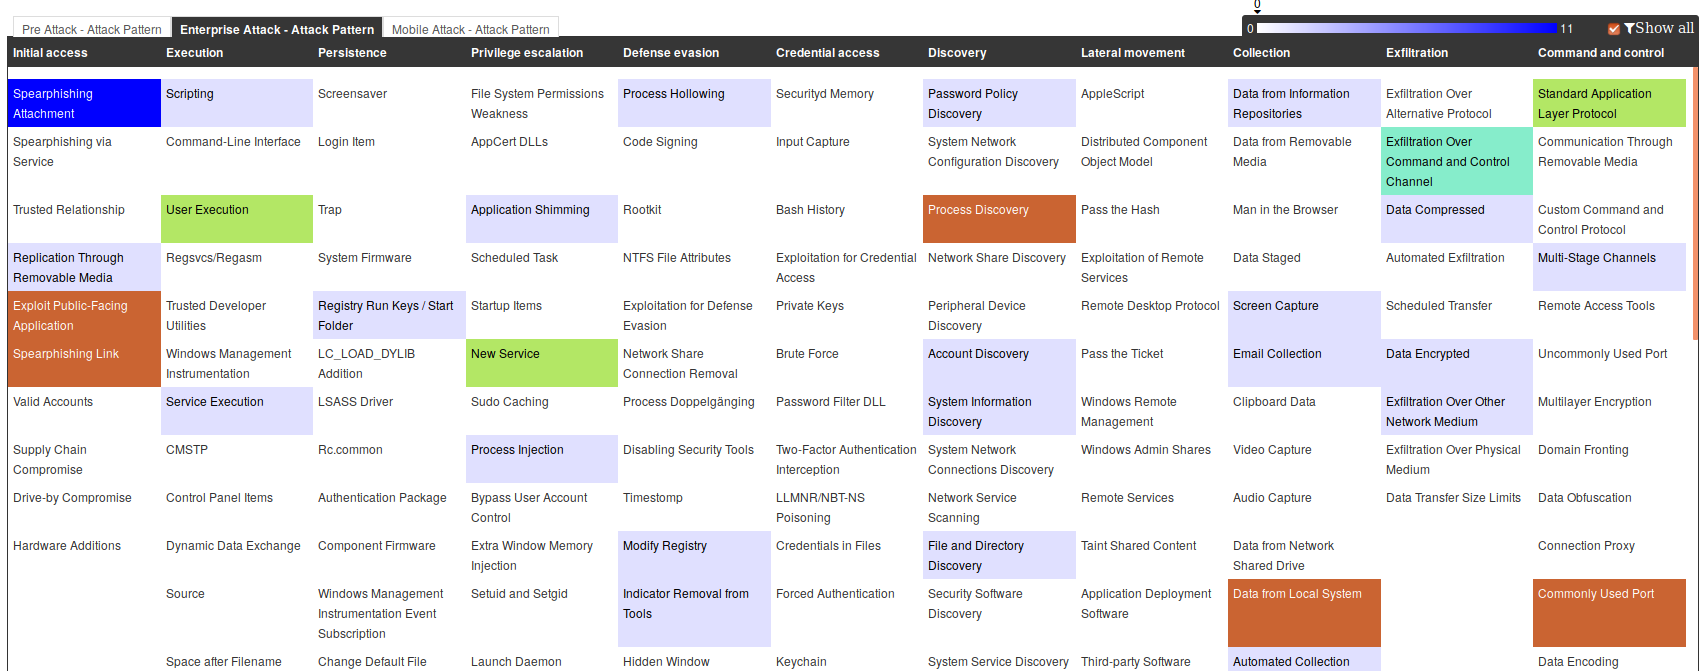
\includegraphics[scale=0.2]{attack-screenshot.png}
  \end{center}
\end{frame}

\begin{frame}
  \frametitle{Monitor trends outside of MISP (example: dashboard)}
  \begin{center}
    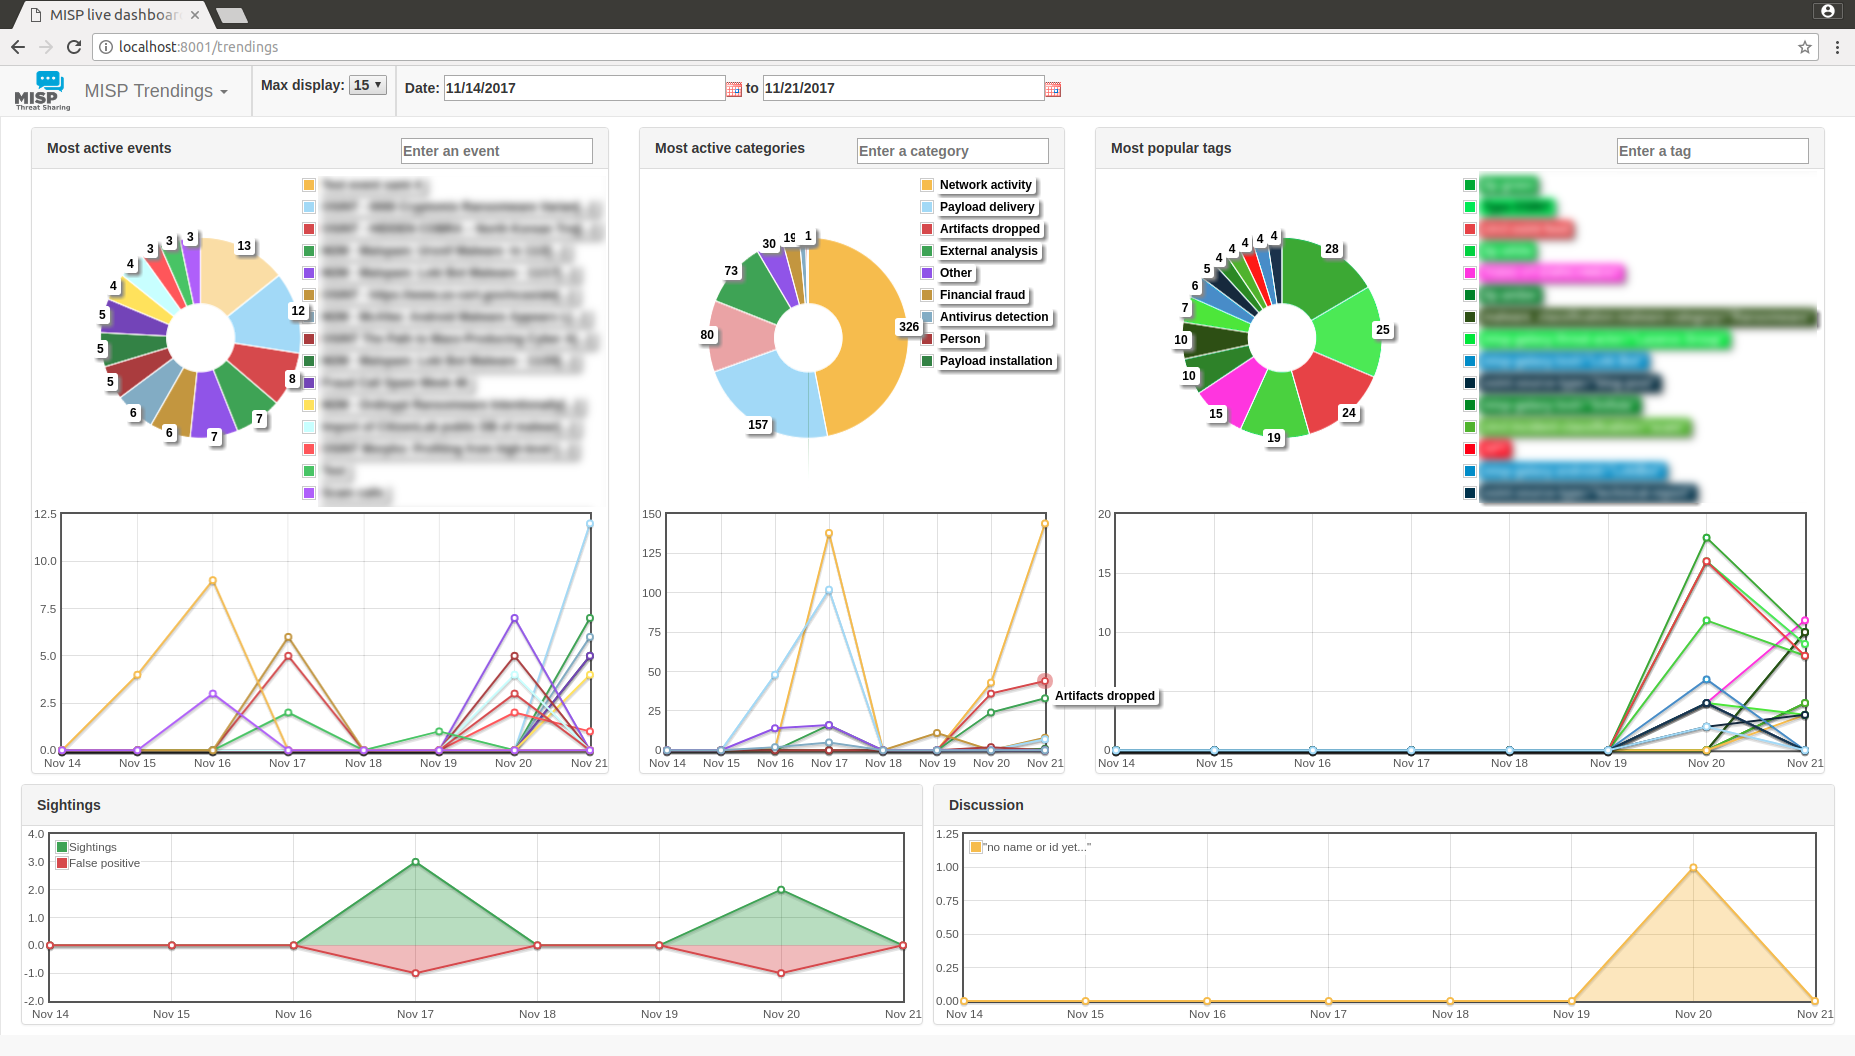
\includegraphics[scale=0.2]{dashboard-trendings.png}
  \end{center}
\end{frame}

\begin{frame}
  \frametitle{Decaying of indicators}
  \begin{itemize}
    \item We were still missing a way to use all of these systems in combination to decay indicators
    \item Move the decision making from complex filter options to complex decay models
    \item Decay models would take into account various taxonomies, sightings, the type of each indicator
    \item The first iteration of what we have in MISP now took:
    \begin{itemize}
       \item 2 years of research
       \item 3 published research papers
       \item A lot of prototyping
    \end{itemize}
  \end{itemize}
\end{frame}

\begin{frame}
    \frametitle{Scoring Indicators: Our solution}
    $$ \texttt{score}(\texttt{\tiny Attribute}) = \texttt{base\_score}(\texttt{\tiny Attribute, Model}) \;\;\bullet\;\; \texttt{decay}(\texttt{\tiny Model, time}) $$
    Where,\vspace{0.5cm}
    \begin{itemize}
        \item \texttt{score} $ \in [0, +\infty $
        \item \texttt{base\_score} $ \in [0, 100] $
        \item \texttt{decay} is a function defined by model's parameters controlling decay speed
        \item \texttt{Attribute} Contains \textit{Attribute}'s values and metadata {\scriptsize (\textit{Taxonomies}, \textit{Galaxies}, ...)}
        \item \texttt{Model} Contains the \textit{Model}'s configuration
    \end{itemize}
\end{frame}

\begin{frame}
    \frametitle{Implementation in MISP: \texttt{Event/view}}
    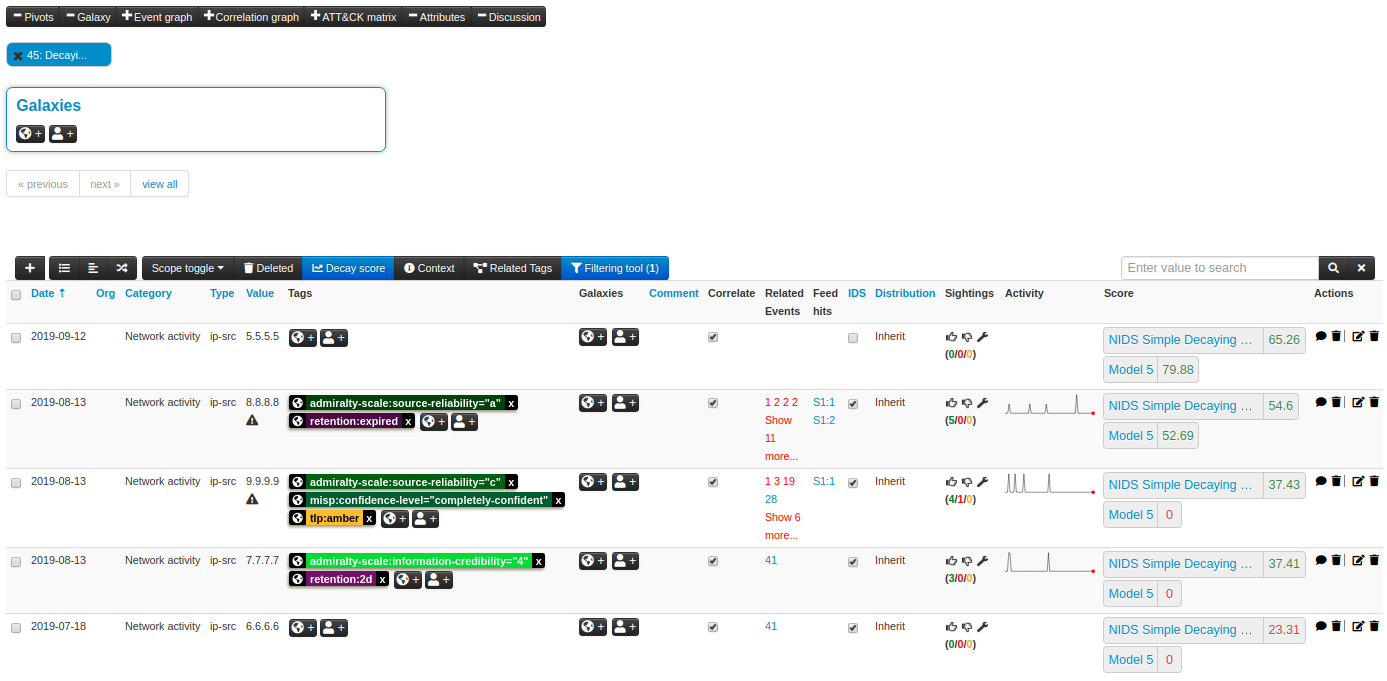
\includegraphics[width=1.00\linewidth]{decaying-event.png}
    \begin{itemize}
        \item \texttt{Decay score} toggle button
        \begin{itemize}
            \item Shows Score for each \textit{Models} associated to the \textit{Attribute} type
        \end{itemize}
    \end{itemize}
\end{frame}

\begin{frame}[fragile]
    \frametitle{Implementation in MISP: API result}
    \texttt{/attributes/restSearch}
    \begin{lstlisting}
"Attribute": [
  {
    "category": "Network activity",
    "type": "ip-src",
    "to_ids": true,
    "timestamp": "1565703507",
    [...]
    "value": "8.8.8.8",
    "decay_score": [
      {
        "score": 54.475223849544456,
        "decayed": false,
        "DecayingModel": {
          "id": "85",
          "name": "NIDS Simple Decaying Model"
        }
      }
    ],
[...]
    \end{lstlisting}
\end{frame}


\begin{frame}
    \frametitle{Implementation in MISP: Index}
    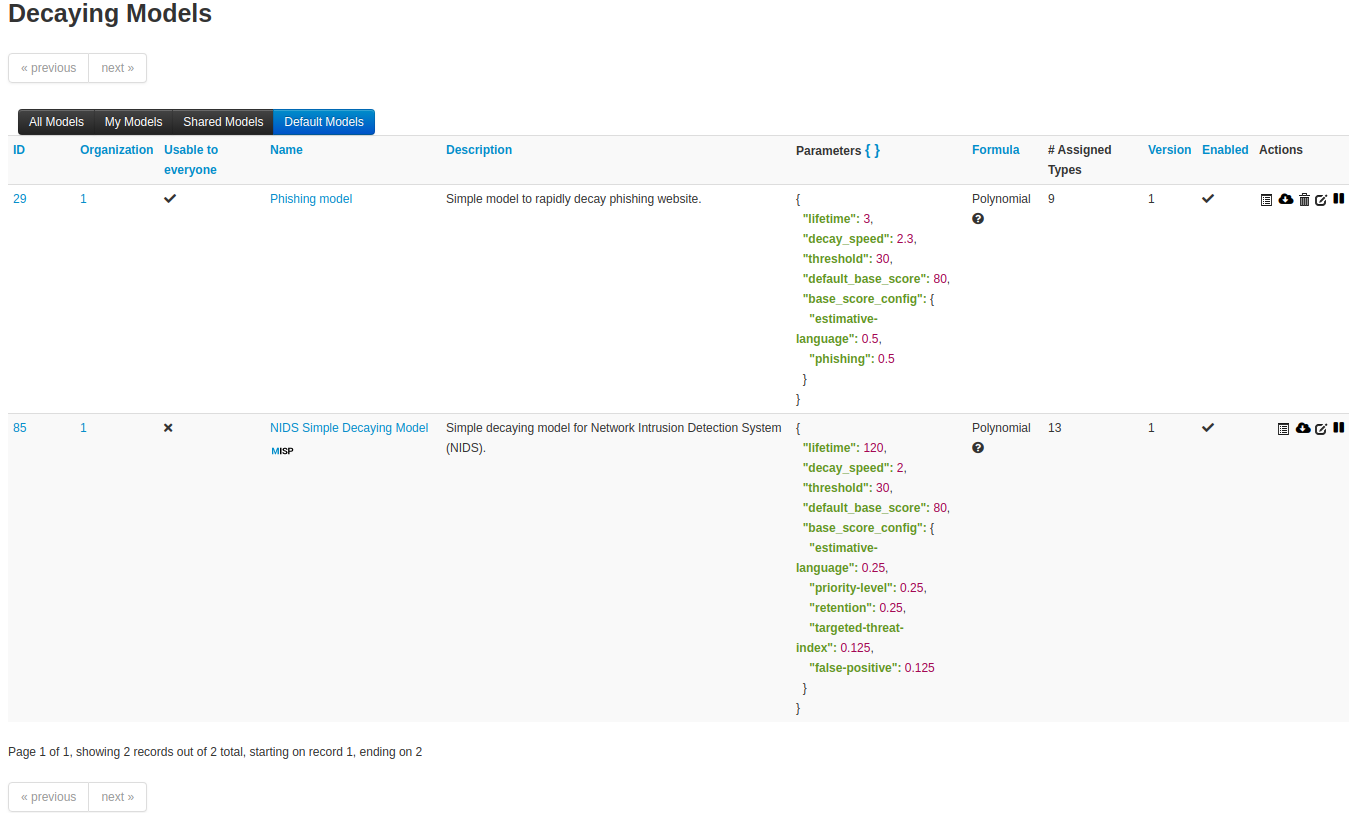
\includegraphics[width=1.00\linewidth]{decaying-index.png}
    View, update, add, create, delete, enable, export, import
\end{frame}

\begin{frame}
    \frametitle{Implementation in MISP: Fine tuning tool}
    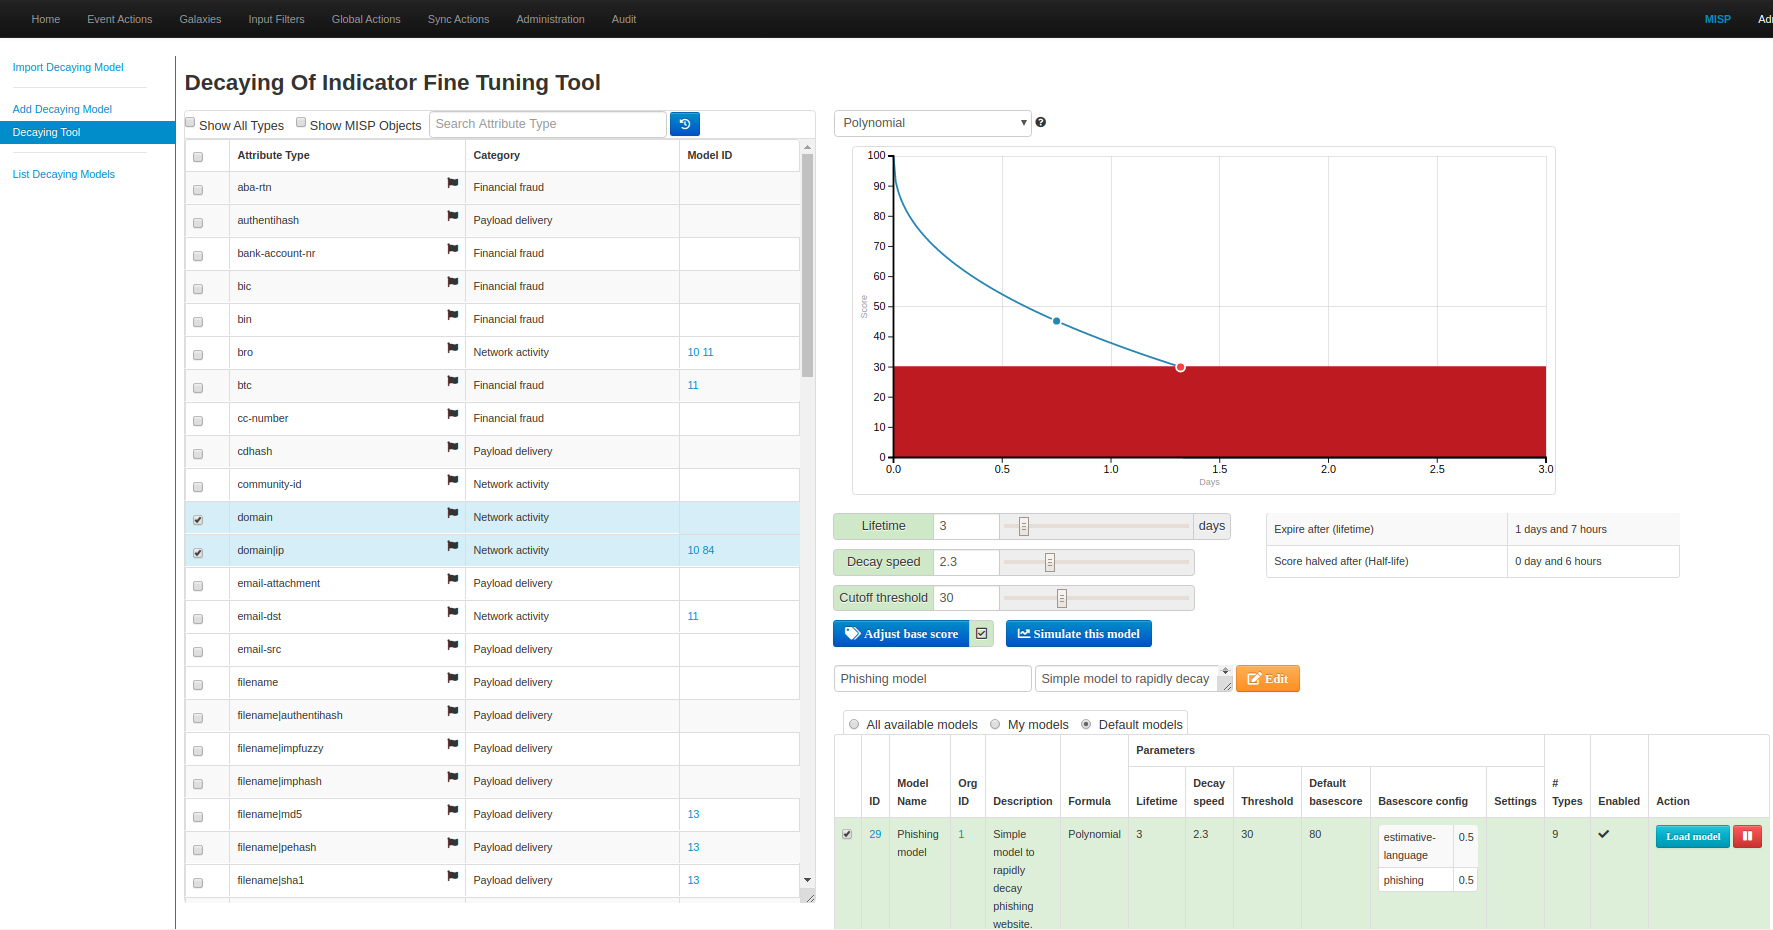
\includegraphics[width=1.00\linewidth]{decaying-tool.png}
    Create, modify, visualise, perform mapping
\end{frame}

\begin{frame}
    \frametitle{Implementation in MISP: \texttt{base\_score} tool}
    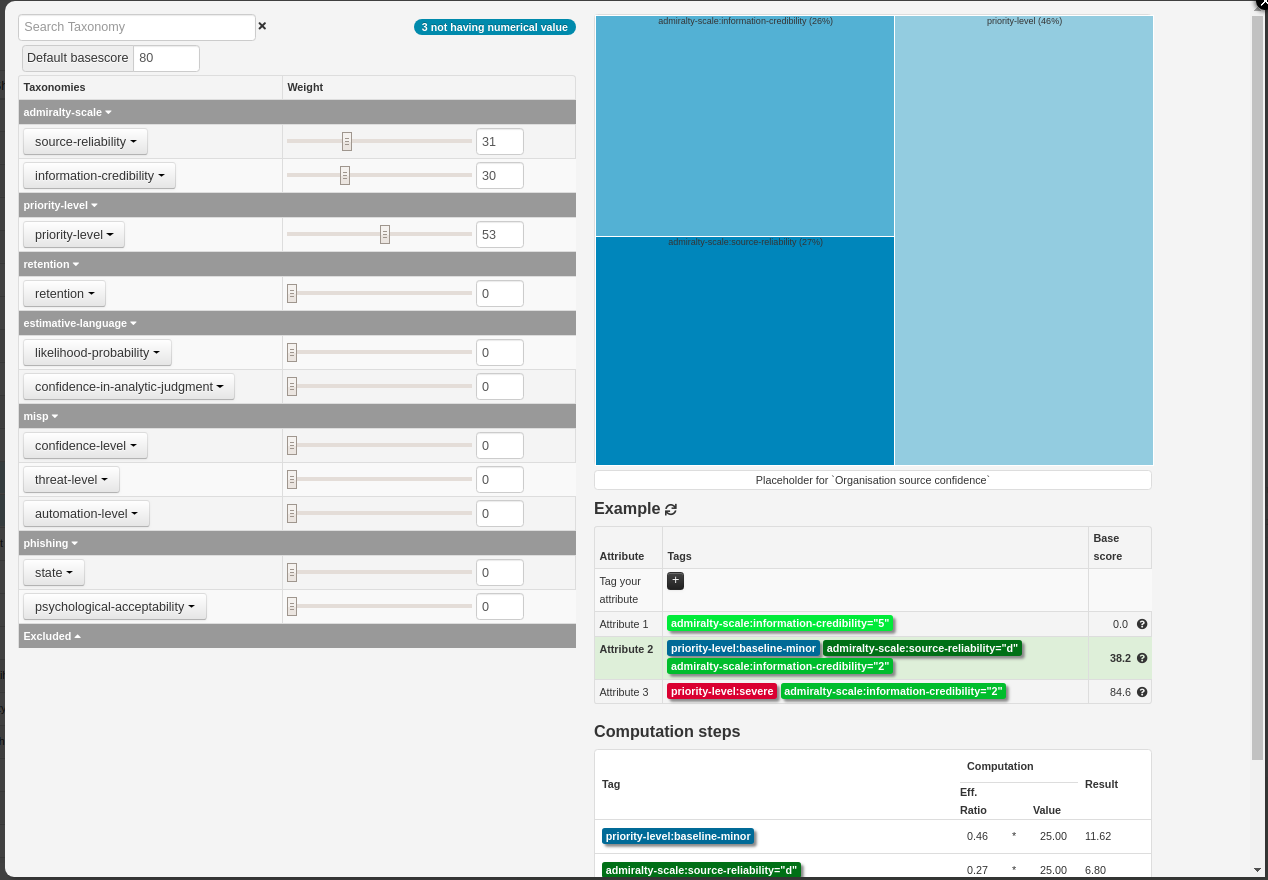
\includegraphics[width=1.00\linewidth]{decaying-basescore.png}
    Adjust Taxonomies relative weights
\end{frame}

\begin{frame}
    \frametitle{Implementation in MISP: simulation tool}
    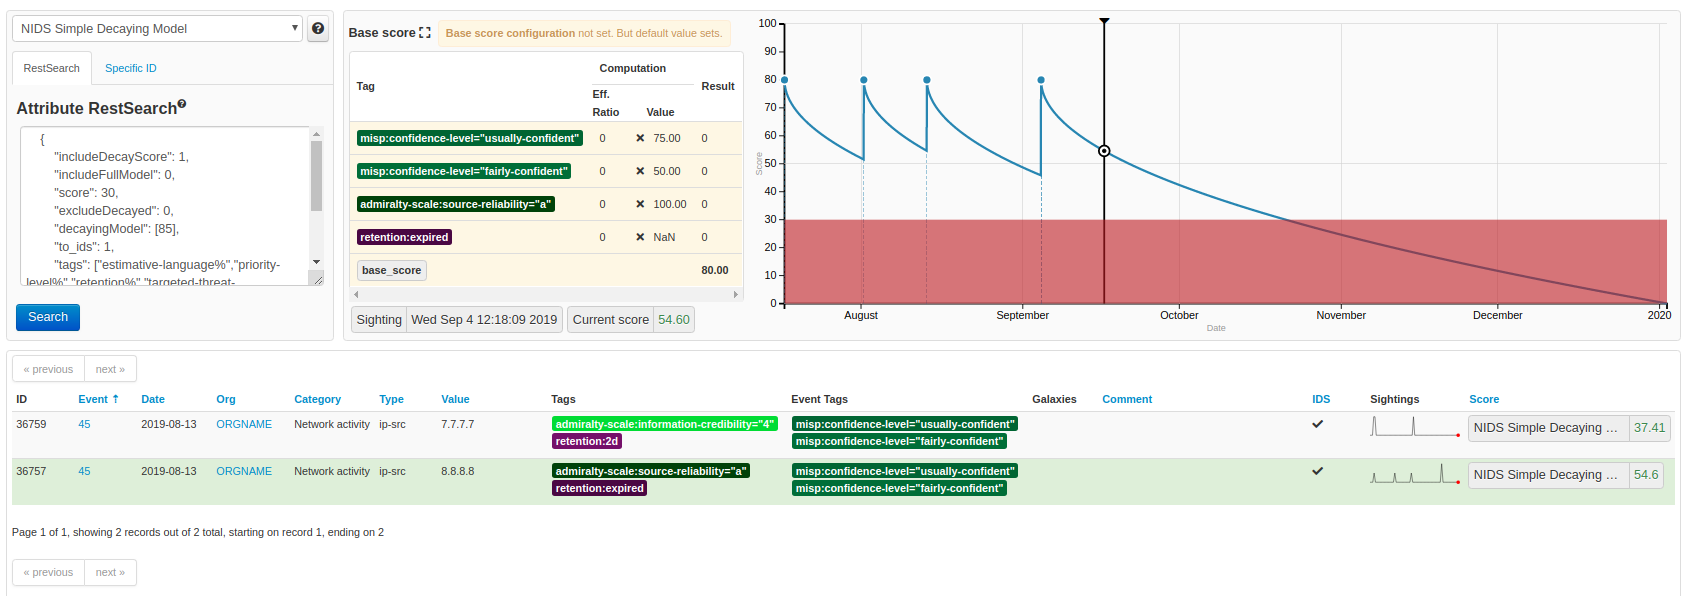
\includegraphics[width=1.00\linewidth]{decaying-simulation.png}
    Simulate \textit{Attributes} with different \textit{Models}
\end{frame}

\begin{frame}[fragile]
    \frametitle{Implementation in MISP: API query body}
    \texttt{/attributes/restSearch}
    \begin{lstlisting}
{
    "includeDecayScore": 1,
    "includeFullModel": 0,
    "excludeDecayed": 0,
    "decayingModel": [85],
    "modelOverrides": {
        "threshold": 30
    }
    "score": 30,
}
    \end{lstlisting}
\end{frame}

\begin{frame}
  \frametitle{Get in touch if you have any questions}
  \begin{itemize}
    \item Contact me
    \begin{itemize}
      \item andras.iklody@circl.lu
      \item \url{https://twitter.com/iglocska}
    \end{itemize}
    \item Contact CIRCL
    \begin{itemize}
      \item info@circl.lu
      \item \url{https://twitter.com/circl_lu}
      \item \url{https://www.circl.lu/}
    \end{itemize}
    \item Contact MISPProject 
    \begin{itemize}
      \item \url{https://github.com/MISP}
      \item \url{https://gitter.im/MISP/MISP}
      \item \url{https://twitter.com/MISPProject}
    \end{itemize}
  \end{itemize}
\end{frame}
